%!TEX root = ../these.tex

\section{Обобщение на задачи сегментной резки SCCP / GSCCP}
\label{sec:ccp.gsccp}

Описанный выше алгоритм разрабатывался и применяется
для решения задачи непрерывной резки CCP,
однако последняя представляет собой весьма
частный случай самой общей формулировки
задачи оптимальной маршрутизации режущего инструмента,
на данный момент это задача прерывистой резки
(Intermittent Cutting Problem, ICP).
Она всё ещё слабо исследована
и представляет существенный научный интерес
как с теоретической точки зрения,
так и в смысле практического использования.

Тогда как задача непрерывной резки возникает фактически
при использовании так называемой
\textit{стандартной техники резки},
существуют и более сложные,
прежде всего
\textit{мульти-сегментная}
и
\textit{мульти-контурная}
техники резки.
Первая характеризуется тем,
что контур детали вырезается в несколько проходов,
с использованием нескольких точек врезки.
Вторая же наоборот, вырезает несколько контуров деталей
за один проход,
как это показано на рис.~\ref{fig:ccp-6x5}.

\begin{figure}
  \centering
  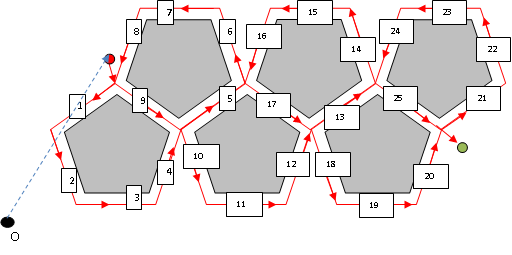
\includegraphics[width=0.95\textwidth]{pentagons.png}
  \caption{Пример составного сегмента резки, содержащего 6 контуров (деталей)}
  \label{fig:ccp-6x5}
\end{figure}

Для включения этих техник в исследование,
полезно расширить понятие контура детали и ввести новый термин:

\textit{Сегмент резки}
$S = \overrightarrow{M M^*}$
--- это часть траектории режущего инструмента от точки врезки $M$
до соответствующей точки выключения инструмента $M^*$.

Сегмент содержит в себе вход в контур
(\textit{lead-in})
и выход из него
(\textit{lead-out}),
а также часть или целый контур детали
или нескольких деталей.
В случае стандартной техники резки
имеется однозначное соответствие между
контурами деталей и сегментами резки,
но в общем случае оно отсутствует.
Фактически, пример мульти-контурной резки на~рис.~\ref{fig:ccp-6x5}
также может представлять собой один единственный
сегмент резки в составе некоторой большой задачи.

Ввиду того,
что сегмент резки по определению содержит в себе
направление резки
(от точки врезки $M$ до точки выключения инструмента $M^*$),
нам потребуется ещё более общее понятие:

\textit{Базовый сегмент}
$B^S$
---
это часть сегмента резки
$S = \overrightarrow{M M^*}$
без участков входа и выхода
(lead-in и lead-out).

Базовый сегмент содержит только геометрию
(части) контуров, подлежащих резке,
и не содержит информации о направлении резки.
